\begin{figure}
    \centering
    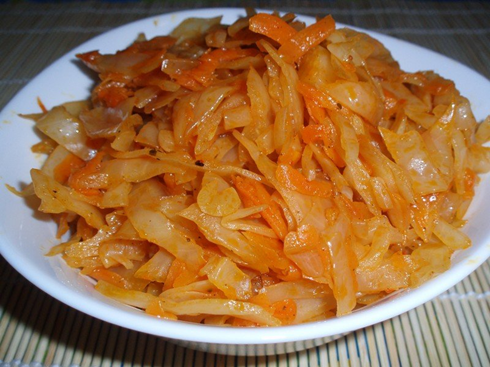
\includegraphics[width=.5\textwidth]{aleksandra/kapusta.png}
\end{figure}

\begin{recipe}
    [ % Optionale Eingaben
        preparationtime = {50 min},
        portion = sehr viel,
        source = Aleksandra
    ]
    {Schmorkohl}

\introduction{
    \# Schmeckt besser als er aussieht
}

\ingredients
{% Zutatenliste
    \unit[1]{} & Kohlkopf \\
    \unit[500]{g} & Sauerkraut \\
    \unit[2]{} & Zwiebeln \\
    \unit[1-2]{} & Möhren   \\    
    \unit[500]{g} & passierte Tomaten \\        
    \unit[2]{} & Zwiebeln \\
     &  Öl       \\
     & Pfeffer \\
    mögl. & Lorbeerblatt \\
    mögl. & Schinkenwürfel / Cranberries \\
}


\preparation
{ % Schrittweise Zubereitung
    \\
    Zwiebel, Möhre schälen, würfeln; Kohl in dünne (etwa Stiftdicke) und längliche (Fingerlang) Streifen schneiden.
    Zwiebeln, Möhren (ggf Schinkenwürfel) im Topf andünsten lassen bis die Zwiebeln glasig werden. \\
    
    Sauerkraut, Kohl in den Topf geben, mit Tomatenmark übergießen, versuchen, umzurühren.\\ 
    
    Etwas Salz, viel Pfeffer dazugeben (ungewöhnlich große Menge, da ungewöhnlich viel Kohl). Die Lorbeerblätter 5-10 Minuten vor Ende dazugeben.
    Schmoren lassen. Der Kohl ist fertig, wenn er zwar nicht mehr knackig ist, aber auch nicht gänzlich labberig. \\
    
    Den Schmorkohl kann man gut als Beilage zu allem essen. Er schmeckt auch kalt. Wenn ich crazy drauf bin, esse ich ihn mit einem Löffel Schmand.    }



\hint
{% Hinweise
    Nimm den größeren Topf.         
}


\end{recipe}
